\documentclass[12pt, dvipsnames, svgnames, x11names,]{article}

\usepackage{xcolor}
% URLs and hyperlinks ---------------------------------------
\usepackage{hyperref}
\hypersetup{
	colorlinks=true,
	linkcolor=NavyBlue,
	filecolor=magenta,      
	urlcolor=blue,
}
\usepackage{xurl}
%---------------------------------------------------
\usepackage[inline]{enumitem}
\usepackage{graphicx}
\usepackage{multirow}
\usepackage{float}
\renewcommand{\arraystretch}{1.40}

% adjust a verrrrry big table -------------------------------
\usepackage{adjustbox}
% -----------------------------------------------------------

\usepackage{array}
% center the p columns and m --------------------------------------------------------------
\newcolumntype{P}[1]{>{\centering\arraybackslash}p{#1}}
\newcolumntype{M}[1]{>{\centering\arraybackslash}m{#1}}
% -------------------------------------------------------------------------------------------------------------

% price
\usepackage{marvosym}
% ----------

\usepackage{xepersian}
\settextfont{Arial}
\setdigitfont{Arial}

\begin{document}
	\begin{titlepage}
		\centering
		\vspace{1cm}
		{\Huge {\textbf{ایندکس معکوس \lr{(Inverted Index)}}}\par}
		\vspace{15mm}
		\vspace{16mm}
		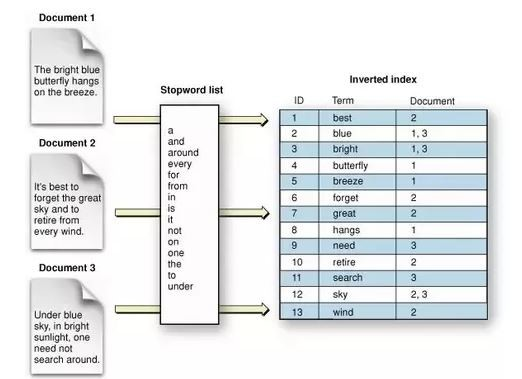
\includegraphics[width=11cm]{images/c0.jpg} \par
		\vfill \par	\vfill
		\vspace{16mm}
		{\normalsize	سیدمحمدحسین هاشمی  4022363143 \par}
		\vspace{1cm}
		{\large فروردین ۱۴۰3\par}
	\end{titlepage}
	\tableofcontents
	\newpage
	
	
	\section{کلاس \lr{Inverted Index}}
	
		{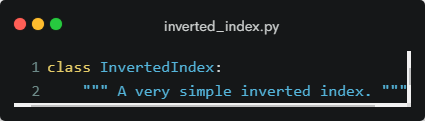
\includegraphics[width=14cm]{images/1.png}}
	
		{\normalsize تمام کدهای مربوطه در این کلاس نوشته می‌شود}
	
				
	
	\section{متد \lr{--init--}}
	
		{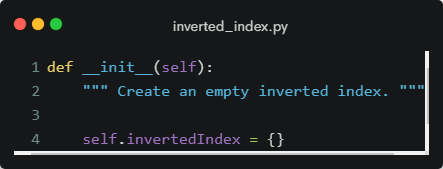
\includegraphics[width=14cm]{images/2.png}} \par
		{\normalsize در اینجا یک دیکشنری خالی برای ذخیره ایندکس‌های معکوس ساخته می‌شود.}
	
	
	\section{متد \lr{read-from-file}}
	
		{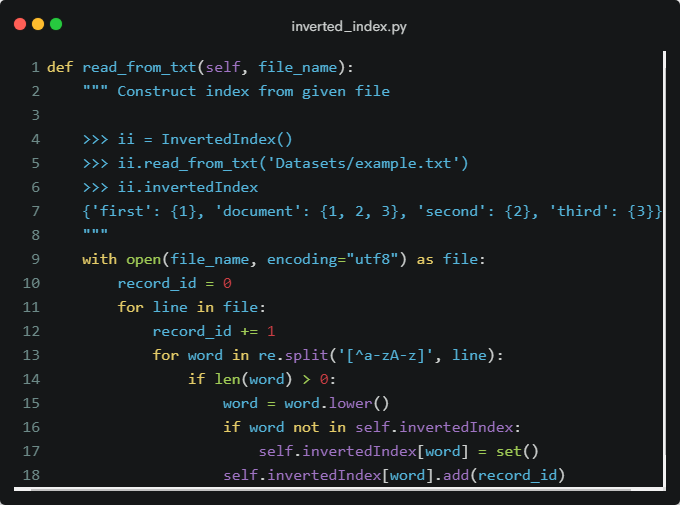
\includegraphics[width=14cm]{images/3.png}} \par
		{\normalsize
			در این متد فایل حاوی متون دریافت و خوانده می‌شود و لازم به ذکر است که تمامی متحوا درون یک خط قرار می‌گیرد.
		} \par

	
	
	\section{متد \lr{search}}
	
		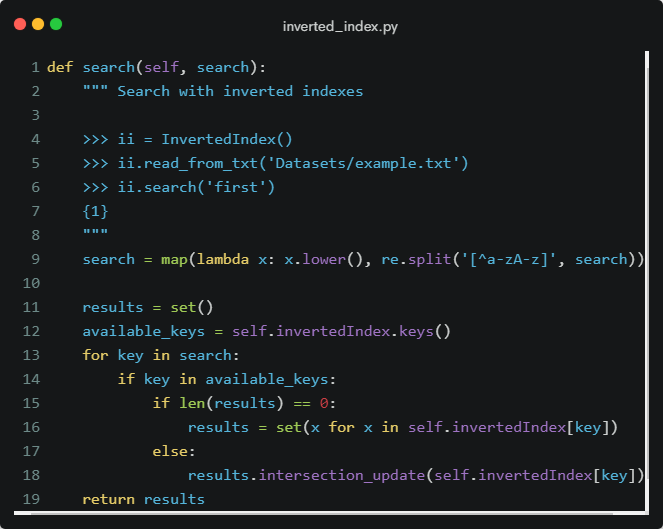
\includegraphics[width=14cm]{images/4.png} \par
		{\normalsize 
			در این متد عملیات اشتراک بین \lr{posting list}ها انجام می‌شود و نتیجه جست‌و‌جو برگشت داده می‌شود.
		}
		
	
	
	\section{خروجی}
	
		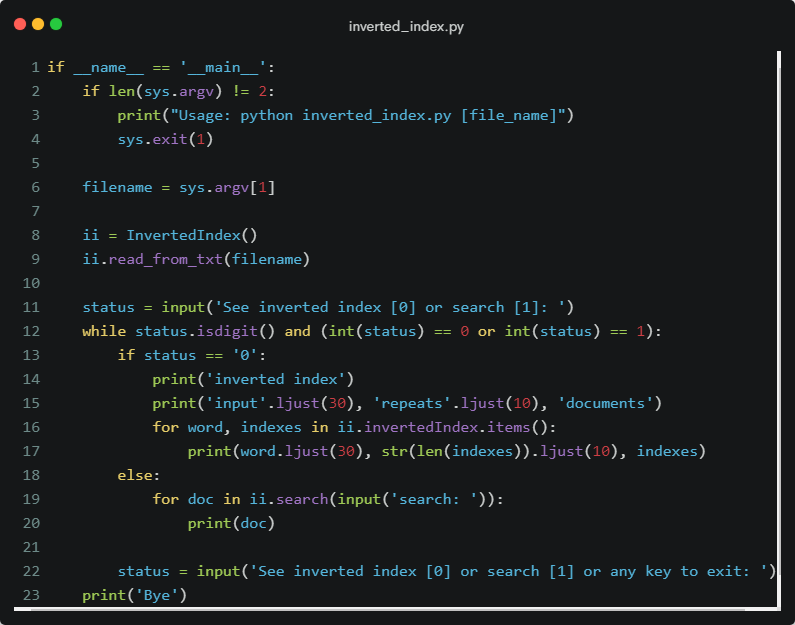
\includegraphics[width=14cm]{images/5.png} \par
		{\normalsize 
			همانطور که مشاهده می‌شود ترمینال ساده ای جهت کارکردن با برنامه ایجاد شده است.
		}		
	
	
\end{document}